\documentclass[man]{apa6}

\usepackage{amssymb,amsmath}
\usepackage{ifxetex,ifluatex}
\usepackage{fixltx2e} % provides \textsubscript
\ifnum 0\ifxetex 1\fi\ifluatex 1\fi=0 % if pdftex
  \usepackage[T1]{fontenc}
  \usepackage[utf8]{inputenc}
\else % if luatex or xelatex
  \ifxetex
    \usepackage{mathspec}
    \usepackage{xltxtra,xunicode}
  \else
    \usepackage{fontspec}
  \fi
  \defaultfontfeatures{Mapping=tex-text,Scale=MatchLowercase}
  \newcommand{\euro}{€}
\fi
% use upquote if available, for straight quotes in verbatim environments
\IfFileExists{upquote.sty}{\usepackage{upquote}}{}
% use microtype if available
\IfFileExists{microtype.sty}{\usepackage{microtype}}{}

% Table formatting
\usepackage{longtable, booktabs}
\usepackage{lscape}
% \usepackage[counterclockwise]{rotating}   % Landscape page setup for large tables
\usepackage{multirow}		% Table styling
\usepackage{tabularx}		% Control Column width
\usepackage[flushleft]{threeparttable}	% Allows for three part tables with a specified notes section
\usepackage{threeparttablex}            % Lets threeparttable work with longtable

% Create new environments so endfloat can handle them
% \newenvironment{ltable}
%   {\begin{landscape}\begin{center}\begin{threeparttable}}
%   {\end{threeparttable}\end{center}\end{landscape}}

\newenvironment{lltable}
  {\begin{landscape}\begin{center}\begin{ThreePartTable}}
  {\end{ThreePartTable}\end{center}\end{landscape}}

  \usepackage{ifthen} % Only add declarations when endfloat package is loaded
  \ifthenelse{\equal{\string man}{\string man}}{%
   \DeclareDelayedFloatFlavor{ThreePartTable}{table} % Make endfloat play with longtable
   % \DeclareDelayedFloatFlavor{ltable}{table} % Make endfloat play with lscape
   \DeclareDelayedFloatFlavor{lltable}{table} % Make endfloat play with lscape & longtable
  }{}%



% The following enables adjusting longtable caption width to table width
% Solution found at http://golatex.de/longtable-mit-caption-so-breit-wie-die-tabelle-t15767.html
\makeatletter
\newcommand\LastLTentrywidth{1em}
\newlength\longtablewidth
\setlength{\longtablewidth}{1in}
\newcommand\getlongtablewidth{%
 \begingroup
  \ifcsname LT@\roman{LT@tables}\endcsname
  \global\longtablewidth=0pt
  \renewcommand\LT@entry[2]{\global\advance\longtablewidth by ##2\relax\gdef\LastLTentrywidth{##2}}%
  \@nameuse{LT@\roman{LT@tables}}%
  \fi
\endgroup}


\ifxetex
  \usepackage[setpagesize=false, % page size defined by xetex
              unicode=false, % unicode breaks when used with xetex
              xetex]{hyperref}
\else
  \usepackage[unicode=true]{hyperref}
\fi
\hypersetup{breaklinks=true,
            pdfauthor={},
            pdftitle={Perceived Grading and Student Evaluation of Instruction},
            colorlinks=true,
            citecolor=blue,
            urlcolor=blue,
            linkcolor=black,
            pdfborder={0 0 0}}
\urlstyle{same}  % don't use monospace font for urls

\setlength{\parindent}{0pt}
%\setlength{\parskip}{0pt plus 0pt minus 0pt}

\setlength{\emergencystretch}{3em}  % prevent overfull lines


% Manuscript styling
\captionsetup{font=singlespacing,justification=justified}
\usepackage{csquotes}
\usepackage{upgreek}

 % Line numbering
  \usepackage{lineno}
  \linenumbers


\usepackage{tikz} % Variable definition to generate author note

% fix for \tightlist problem in pandoc 1.14
\providecommand{\tightlist}{%
  \setlength{\itemsep}{0pt}\setlength{\parskip}{0pt}}

% Essential manuscript parts
  \title{Perceived Grading and Student Evaluation of Instruction}

  \shorttitle{Perceived Grading and Student Evaluation}


  \author{Erin M. Buchanan\textsuperscript{1}, Becca N. Huber\textsuperscript{1, 2}, Arden Miller\textsuperscript{1}, David W. Stockburger\textsuperscript{3}, \& Marshall Beauchamp\textsuperscript{4}}

  \def\affdep{{"", "", "", "", ""}}%
  \def\affcity{{"", "", "", "", ""}}%

  \affiliation{
    \vspace{0.5cm}
          \textsuperscript{1} Missouri State University\\
          \textsuperscript{2} Idaho State University\\
          \textsuperscript{3} US Air Force Academy\\
          \textsuperscript{4} University of Missouri - Kansas City  }

  \authornote{
    \newcounter{author}
    A portion of this research was presented at the meeting of the
    Southwestern Psychological Association, April, 2009, San Antonio, TX.
    The authors would like to thank Melissa Fallone for comments on earlier
    drafts and Stephen Martin for his help with restructuring the data.

                      Correspondence concerning this article should be addressed to Erin M. Buchanan, 901 S. National Ave, Springfield, MO, 65897. E-mail: \href{mailto:erinbuchanan@missouristate.edu}{\nolinkurl{erinbuchanan@missouristate.edu}}
                                                        }


  \abstract{We analyzed student evaluations for 3,585 classes collected over 20
years to determine stability and evaluate the relationship of perceived
grading to global evaluations, perceived fairness, and appropriateness
of assignments. Using class as the unit of analysis, we found small
evaluation reliability when professors taught the same course in the
same semester, with much weaker correlations for differing courses.
Expected grade and grading related questions correlated with overall
evaluations of courses. Differences in course evaluations on expected
grades, grading questions, and overall grades were found between
full-time faculty and other types of instructors. These findings are
expanded to a model of grading type questions mediating the relationship
between expected grade and overall course evaluations with a moderating
effect of type of instructor.}
  \keywords{Student evaluation, teacher evaluation, perceived grading, reliability \\

    
  }





\usepackage{amsthm}
\newtheorem{theorem}{Theorem}
\newtheorem{lemma}{Lemma}
\theoremstyle{definition}
\newtheorem{definition}{Definition}
\newtheorem{corollary}{Corollary}
\newtheorem{proposition}{Proposition}
\theoremstyle{definition}
\newtheorem{example}{Example}
\theoremstyle{definition}
\newtheorem{exercise}{Exercise}
\theoremstyle{remark}
\newtheorem*{remark}{Remark}
\newtheorem*{solution}{Solution}
\begin{document}

\maketitle

\setcounter{secnumdepth}{0}



Student evaluations of professors are a typical practice, but their
validity and reliability has been disputed. The impact of student
evaluations on professor advancement can be great and often acts as a
deciding factor in professor promotion, demotion, coursework choice,
tenureship, or to inform access to certain funding opportunities. Some
suggest that there are variables that result in improving evaluations,
such as giving higher grades (Greenwald \& Gillmore, 1997; Isely \&
Singh, 2005; Krautmann \& Sander, 1999). Student evaluations are also
influenced by likability, attractiveness, and dress (Buck \& Tiene,
1989; Gurung \& Vespia, 2007; Hugh Feeley, 2002). Further, 20 years ago,
Neath (1996) suggested twenty tongue-in-cheek tips in which professors
may bolster their evaluations from students. These suggestions have no
relationship with research supported instructional methods or further
learning retention among the student body, such as being a male
professor and only teaching only male students. In more recent research,
Boring, Ottoboni, \& Stark (2016) confirms that student evaluations of
teaching are biased against female instructors, and the authors conclude
student evaluations are more representative of the students' grading
expectations and biases rather than an evaluation of objective
instructional methods. All together, these findings elicit the argument
that student evaluations are not necessarily measuring whether the
instructional methods of professors are sound, rather student
evaluations of instruction are measuring whether or not the instructor
met the students' expectations of their performance in the classroom, in
addition to the instructor meeting pre-existing biases.

However, this finding does not imply that an instructor can simply raise
grades to meet expectations (Centra, 2003; Marsh, 1987; Marsh \& Roche,
2000), instead one should consider the effect of \enquote{perceived
grading}. We operationally define perceived grading as the students'
perceptions of assignment appropriateness, grading fairness, and the
expected course grade at the time the evaluations are being completed.
Social psychology theory would support that students with low perceived
grading perceptions may reduce cognitive dissonance and engage in ego
defense by giving low evaluations in turn (Maurer, 2006), subsequently
resulting in decreased validity and reliability of the proposed
construct, professor instruction. We argue both social psychology theory
and the evidence from student evaluations supports that higher perceived
grading can lead to better student evaluations of instruction. For
example, Salmons (1993) provided causal evidence of lowered student
evaluations due to expected grades. In her study of 444 students
completing faculty evaluations at two separate points in a semester,
students who expected to get Fs significantly lowered their evaluations
while students who expected to receive As and Bs significantly raised
their evaluations (Salmons, 1993). This theory and evidence from student
evaluation leads us to further argue student evaluations of professors
are biased towards their expected grade and the perceived fairness of
the grading system, rather than the actual instructional methods used
over the course of a semester.

Much of the literature on student evaluations involves diverse and
complex analyses (e.g., Marsh (1987)) and lacks social-psychological
theoretical guidance on human judgment. To expect that student
evaluations would not be influenced by expected grade would contradict a
long-standing history of social psychology research on cognitive
dissonance, attribution, and ego threat. As we know, failure threatens
the ego (Miller, 1985) and motivates us to find rationales to defend the
ego. Further, Kenworthy, Miller, Collins, Read, \& Earleywine (2011)
found guilt as a significant correlate of dissonance which may be
illuminated in this study by the guilt of under-performing from a
student's own expectations. Failing students, or those performing below
personal expectations, would be expected to defend their ego by
attributing low grades to poor teaching or unfair evaluation practices
(Maurer, 2006). One common strategy involves diminishing the value of
the activity (Miller \& Klein, 1989), which would result in lowered
perceived value of a course.

Similarly, Cognitive Dissonance Theory (Festinger, 1957) predicts that
people who experience poor performance but perceive themselves as
competent will experience dissonance, of which they can reduce through
negative evaluations of the instruction (Maurer, 2006). Attribution
research (Weiner, 1992) also supports the argument that among low
achievement motivation students, failure is associated with external
attributions for cause, and the most plausible external attribution for
the student in the evaluation context is the quality of instruction and
grading practices. Although arguments regarding degree of influence are
reasonable, the position that they are not affected is inconsistent with
existing and established theory. Thus, it is not surprising that the
majority of faculty perceive student evaluations to be biased by
perceived grading and course choice (Marsh, 1987).

Blackhart, Peruche, DeWall, \& Joiner (2006) analyzed 167 psychology
classes in a multiple regression analysis and found the two most
significant predictors of instructor ratings were average grade given by
the instructor and instructor status (teaching assistant or ranked
faculty). Because of the limited number of classes, the power of the
analysis was limited. However, in addition to the concern regarding the
relationship between grades and global course evaluations, it was found
that teaching assistants were rated more highly than ranked faculty.
This finding raises additional questions on validity student evaluation
of instructional quality. We must either accept that the least trained
and qualified instructors are actually better teachers, or we must
believe this result suggests that student evaluations have given us
false information on the quality of instruction via their perceptions of
grading. Research from DuCette \& Kenney (1982) and Ellis, Burke,
Lomire, \& McCormack (2003) also showed medium to large correlations
between expected grade and course ratings. However, these studies did
not consider the predictive relationship for instructors across
different courses and semesters, which was one aim of the current study.
Using nearly twenty years of data from a large midwestern university,
the following research questions were examined:

\begin{enumerate}
\def\labelenumi{\arabic{enumi})}
\item
  If ratings are, in fact, valid measures of instructor attributes, it
  should be expected that ratings would have some stability across
  semesters and specific courses. If variation were due to instructor
  attributes and not the course they are assigned, we would expect
  ratings to be most stable across two different courses during the same
  semester. We would expect these correlations to decline somewhat for
  the same course in a different semester, since faculty members may
  improve or decline with experience. However, if they are reliable and
  stable enough to use in making choices about retention, their
  stability should be demonstrated across different semesters, as well.
  Therefore, in the current study, we first sought to establish if
  ratings are reliable for instructors across courses and semesters.
  This analysis was conducted by calculating all possible correlations
  between each average course rating in the dataset to examine course
  (same/different) by semester (same/different) by instructor
  (same/different) reliability.
\item
  After examining reliability, we sought to show that items on
  instructor evaluations were positively correlated, demonstrating that
  overall course evaluations are related to perceived grading ratings
  from the students.
\item
  Given the proposed differences in ratings by instructor type
  (Blackhart et al., 2006), we examined a moderated mediation analysis
  to portray the expected relationship of the variables across
  instructor type. First, for the mediation analysis, we hypothesized
  that expected grade predicted overall course rating, with perceived
  grading ratings mediating that relationship. With this analysis, we
  would demonstrate that evaluations are not merely a measure of
  expected grade, but also influenced by grading system used in the
  course (i.e., students with higher grades likely perceive grading to
  be more fair/appropriate, which then influences their ratings of the
  course). This mediation was expected to be moderated by instructor
  type, as previous research has shown that different types of
  instructors (teaching assistants, ranked faculty) appear to receive
  different ratings overall.
\end{enumerate}

\section{Method}\label{method}

The archival study was conducted using data from the psychology
department at a large Midwestern public university. We used data from
4313 undergraduate, 397 mixed-level undergraduate, and 687 graduate
psychology classes taught from 1987 to 2016 that were evaluated by
students using the same 15-item instrument. The graduate courses were
excluded from analyses due to the ceiling effects on expected grades.
Faculty followed set procedures in distributing scan forms no more than
two weeks before the conclusion of the semester. A student was assigned
to collect the forms and deliver them to the departmental secretary. The
instructor was required to leave the room while students completed the
forms.

We focused upon the five items, which seemed most pertinent to the
issues of perceived grading and evaluation. We were most interested in
how grades related to global course evaluation and grading/assignment
evaluations. These items were presented with a five-point scale from 1
(\emph{strongly disagree}) to 5 (\emph{strongly agree}):

\begin{enumerate}
\def\labelenumi{\arabic{enumi})}
\tightlist
\item
  The overall quality of this course was among the top 20\% of those I
  have taken.
\item
  The examinations were representative of the material covered in the
  assigned readings and class lectures.
\item
  The instructor used fair and appropriate methods in the determination
  of grades.
\item
  The assignments and required activities in this class were
  appropriate.
\item
  What grade do you expect to receive in this course? (A = 5, B, C, D, F
  = 1).
\end{enumerate}

\section{Results}\label{results}

All data were checked for course coding errors, and type of instructor
was coded as graduate teaching assistant, per-course faculty, full-time
instructors, and tenure-track faculty. Graduate teaching assistants were
generally assigned to teach lower-level introductory courses
(Introduction to Psychology, Statistics for Psychology, Research Methods
laboratories), and these students were interviewed and hired by the
faculty supervising those courses. Graduate students were generally in
their second year of the masters program in the department, and levels
of supervision varied by course and supervisor.

This data was considered structured by instructor; therefore, all
analyses below were coded in \emph{R} using the \emph{nlme} package
(Pinheiro, Bates, Debroy, Sarkar, \& Team, 2017) to control for
correlated error of instructor as a random intercept in a multilevel
model. Multilevel models allow for analysis of repeated measures data
without collapsing by participant (i.e., each instructor/semester/course
combination can be kept separate without averaging over these
measurements; Gelman, 2006). Random intercept models are regression
models on the repeated data that structure the data by a specified
variable, which was instructor in this analysis. Therefore, each
instructor's average rating score was allowed to vary within the
analysis, as ratings would be expected to be different from instructor
to instructor. In each of the analyses described below, the number of
students providing ratings for the course was included as a control
variable to even out differences in course size as an influence in the
results. The dependent variable and predictors varied based on the
research question, and these are described with each analysis below.

The overall dataset was screened for normality, linearity, homogeneity,
and homoscedasticity using procedures from Tabachnick \& Fidell (2012).
Data generally met assumptions with a slight skew and some
heterogeneity. This data was not screened for outliers because it was
assumed that each score was entered correctly from student evaluations.
The complete set of all statistics can be found online at
\url{http://osf.io/jdpfs}. This page also includes the manuscript
written inline with the statistical analysis with the \emph{papaja}
package (Aust \& Barth, 2017) for interested researchers/reviewers who
wish to recreate these analyses.

\subsection{Reliability of Instructor
Scores}\label{reliability-of-instructor-scores}

\begin{table}[tbp]
\begin{center}
\begin{threeparttable}
\caption{\label{tab:rel-table}Correlations for Instructor, Semester, and Course Combinations}
\small{
\begin{tabular}{lllccccc}
\toprule
Instructor & Semester & Course & $b$ & $SE$ & $df$ & $t$ & $p$\\
\midrule
Different Instructor & Different Semester & Different Course & -.001 & .000 & 10144295 & -3.580 & .013\\
Different Instructor & Same Semester & Different Course & .006 & .002 & 152801 & 2.906 & .048\\
Different Instructor & Different Semester & Same Course & .008 & .001 & 517353 & 6.236 & .027\\
Different Instructor & Same Semester & Same Course & .054 & .010 & 6265 & 5.402 & < .001\\
Same Instructor & Different Semester & Different Course & -.038 & .003 & 108849 & -13.130 & < .001\\
Same Instructor & Same Semester & Different Course & .095 & .020 & 1872 & 4.659 & < .001\\
Same Instructor & Different Semester & Same Course & .090 & .004 & 55057 & 21.769 & < .001\\
Same Instructor & Same Semester & Same Course & .446 & .023 & 1401 & 19.631 & < .001\\
\bottomrule
\end{tabular}
}
\end{threeparttable}
\end{center}
\end{table}

Reliability of ratings of instructors can be inferred by the consistency
of ratings across courses and semester, assuming that we infer there is
a stable good/poor instructor attribute and that these multiple
administrations of the same question are multiple assessments of that
attribute. A file was created with all possible course pairings for
every instructor, semester, and course combination. Therefore, this
created eight possible combinations of matching v. no match for
instructor by semester by course. Multilevel models were used to
calculate correlations on each of the eight combinations controlling for
response size for both courses (i.e., course 1 number of ratings and
course 2 number of ratings) and random intercepts for instructor(s). The
independent variable was the question rating for one
instructor/semester/course combination, while the dependent variable was
the same question rating for a second combination. The target variable
of interest was therefore the correlation between these two ratings,
after adjusting for individual differences due to instructor (random
intercepts) and course size (control variable). Correlations were
calculated separately for each of the target questions listed above.

The overall pattern of the data was the same for each of the eight
combinations, and these were averaged for Table \ref{tab:rel-table}. The
complete set of all correlations can be found online. Given that the
large sample size would bias statistical significance based on
\emph{p}-values, we focused on the size of the correlations. The
correlations were largest for the same instructor in the same semester
and course, followed by the same instructor in the same semester with a
different course and the same instructor in a different semester with
the same course. The first shows that scores are somewhat reliable
(i.e., \emph{r}s \textasciitilde{} .45) for instructors teaching two or
more of the same class at the same time. The correlations within
instructor then drop to \emph{r}s \textasciitilde{} .09 for the same
semester or same course. All other correlations are nearly zero, with
the same semester, same course, and different instructor as the next
largest at \emph{r}s \textasciitilde{} .05. Given these values are still
low for traditional reliability standards, these results may indicate
that student demand characteristics or course changes impact instructor
ratings.

\subsection{Correlations of Evaluation
Questions}\label{correlations-of-evaluation-questions}

\begin{table}[tbp]
\begin{center}
\begin{threeparttable}
\caption{\label{tab:correlation-table}t Statistics for Inter-item Relationship}
\begin{tabular}{lcccccc}
\toprule
Coefficient & $pr$ & $b$ & $SE$ & $df$ & $t$ & $p$\\
\midrule
Overall to Exams & .637 & .828 & .014 & 4447 & 60.813 & < .001\\
Overall to Fair & .606 & .903 & .016 & 4447 & 57.837 & < .001\\
Overall to Assignments & .675 & .999 & .016 & 4447 & 63.251 & < .001\\
Overall to Expected Grade & .344 & .597 & .022 & 4447 & 27.167 & < .001\\
Exams to Fair & .655 & .751 & .012 & 4447 & 61.387 & < .001\\
Exams to Assignments & .615 & .700 & .014 & 4447 & 50.425 & < .001\\
Exams to Expected Grade & .311 & .416 & .018 & 4447 & 23.066 & < .001\\
Fair to Assignments & .720 & .715 & .011 & 4447 & 63.912 & < .001\\
Fair to Expected Grade & .375 & .438 & .016 & 4447 & 27.865 & < .001\\
Assignments to Expected Grade & .344 & .404 & .015 & 4447 & 26.913 & < .001\\
\bottomrule
\end{tabular}
\end{threeparttable}
\end{center}
\end{table}

In this analysis, we correlated each of the five relevant evaluation
questions, as the above analysis indicated reliability for each item
across time, but not their relation to each other. The multilevel models
for this analysis included course size as an adjustor variable, one
evaluation item as the independent variable, and a separate evaluation
item as the dependent variable. Again, these included the instructor as
a random intercept to control for differences in average ratings. This
analysis was on the original dataset where each
semester/course/instructor combination was only compared to the matching
semester/course/instructor combination (i.e., ratings are correlated
only on the exact same course, semester, and instructor), rather than
the special dataset created above for reliability.

Table \ref{tab:correlation-table} presents the inter-correlations for
the five relevant evaluation questions. The partial correlation
(\emph{pr}) is the standardized coefficient from the multilevel model
analysis between items while adjusting for sample size and random
effects of instructor. The raw coefficient \emph{b}, standard error, and
significance statistics are also provided. We found class expected grade
was related to class overall rating, exams reflecting the material,
grading fairness, and appropriateness of assignments; however, these
partial correlations were approximately half of all other pairwise
correlations. The correlations between grading related items were high,
representing some consistency in evaluation, as well as the overall
course evaluation to grading questions.

\subsection{Moderated Mediation}\label{moderated-mediation}

\begin{figure}
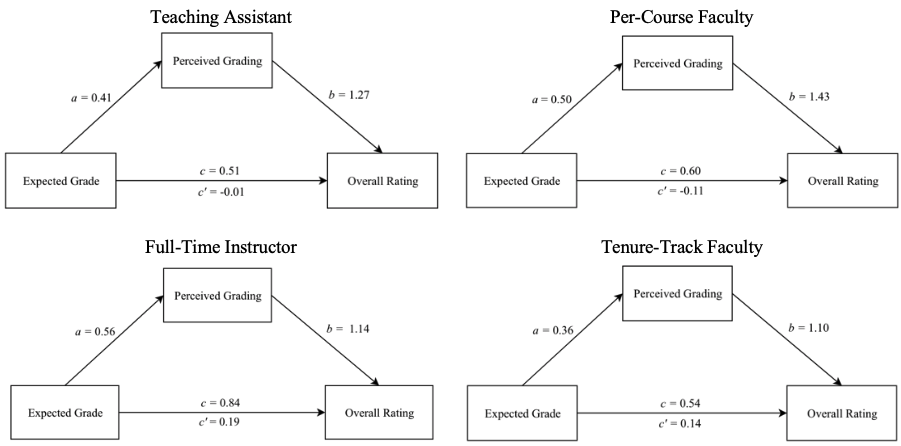
\includegraphics[width=7in,height=5in]{complete_medmod} \caption{Mediation models for moderated mediation analysis indicating mediation effects for each type of teacher. Expected grading indicates student entered grade expected in the course, perceived grading is an average score of fairness, appropriateness, and exam grading questions, and overall rating indicates the omnibus rating for a course.}\label{fig:med-mod-pic}
\end{figure}

\begin{table}[tbp]
\begin{center}
\begin{threeparttable}
\caption{\label{tab:table-mod-med}t Statistics for Moderated Mediation}
\small{
\begin{tabular}{llccccc}
\toprule
DV & IV & $b$ & $SE$ & $df$ & $t$ & $p$\\
\midrule
Overall Course & Expected Grade & 0.493 & 0.102 & 4336 & 4.857 & < .001\\
Overall Course & Teaching Assistant & 0.114 & 0.085 & 191 & 1.345 & .180\\
Overall Course & Per-Course & -0.102 & 0.116 & 191 & -0.880 & .380\\
Overall Course & Instructor & 0.096 & 0.081 & 191 & 1.187 & .237\\
Overall Course & EG X TA & 0.126 & 0.126 & 4336 & 0.996 & .319\\
Overall Course & EG X PC & 0.304 & 0.115 & 4336 & 2.637 & .008\\
Overall Course & EG X IN & 0.049 & 0.105 & 4336 & 0.464 & .643\\
Average Grading & Expected Grade & 0.416 & 0.062 & 4336 & 6.667 & < .001\\
Average Grading & Teaching Assistant & -0.023 & 0.047 & 191 & -0.492 & .623\\
Average Grading & Per-Course & -0.132 & 0.063 & 191 & -2.096 & .037\\
Average Grading & Instructor & -0.083 & 0.044 & 191 & -1.860 & .064\\
Average Grading & EG X TA & 0.111 & 0.078 & 4336 & 1.428 & .153\\
Average Grading & EG X PC & 0.117 & 0.071 & 4336 & 1.642 & .101\\
Average Grading & EG X IN & -0.056 & 0.064 & 4336 & -0.870 & .384\\
Overall Course & Expected Grade & -0.024 & 0.077 & 4332 & -0.313 & .755\\
Overall Course & Teaching Assistant & 0.142 & 0.048 & 191 & 2.936 & .004\\
Overall Course & Per-Course & 0.065 & 0.063 & 191 & 1.028 & .305\\
Overall Course & Instructor & 0.198 & 0.045 & 191 & 4.388 & < .001\\
Overall Course & Average Grading & 1.241 & 0.085 & 4332 & 14.583 & < .001\\
Overall Course & EG X TA & -0.126 & 0.098 & 4332 & -1.283 & .200\\
Overall Course & EG X PC & 0.206 & 0.091 & 4332 & 2.271 & .023\\
Overall Course & EG X IN & 0.173 & 0.080 & 4332 & 2.164 & .031\\
Overall Course & AG X TA & 0.216 & 0.103 & 4332 & 2.107 & .035\\
Overall Course & AG X PC & -0.081 & 0.099 & 4332 & -0.821 & .412\\
Overall Course & AG X IN & -0.142 & 0.087 & 4332 & -1.634 & .102\\
\bottomrule
\end{tabular}
}
\end{threeparttable}
\end{center}
\end{table}

\begin{table}[tbp]
\begin{center}
\begin{threeparttable}
\caption{\label{tab:table-med-split}t Statistics for Individual Mediations}
\small{
\begin{tabular}{lllccccc}
\toprule
Group & DV & IV & $b$ & $SE$ & $df$ & $t$ & $p$\\
\midrule
Teaching Assistant & Overall Course & Expected Grade & 0.510 & 0.092 & 219 & 5.534 & < .001\\
Teaching Assistant & Average Grading & Expected Grade & 0.407 & 0.049 & 219 & 8.326 & < .001\\
Teaching Assistant & Overall Course & Expected Grade & -0.010 & 0.077 & 218 & -0.126 & .900\\
Teaching Assistant & Overall Course & Average Grading & 1.265 & 0.084 & 218 & 15.017 & < .001\\
Per-Course & Overall Course & Expected Grade & 0.605 & 0.071 & 425 & 8.536 & < .001\\
Per-Course & Average Grading & Expected Grade & 0.505 & 0.040 & 425 & 12.640 & < .001\\
Per-Course & Overall Course & Expected Grade & -0.109 & 0.051 & 424 & -2.163 & .031\\
Per-Course & Overall Course & Average Grading & 1.426 & 0.049 & 424 & 28.991 & < .001\\
Instructor & Overall Course & Expected Grade & 0.836 & 0.054 & 504 & 15.511 & < .001\\
Instructor & Average Grading & Expected Grade & 0.562 & 0.035 & 504 & 15.967 & < .001\\
Instructor & Overall Course & Expected Grade & 0.194 & 0.044 & 503 & 4.375 & < .001\\
Instructor & Overall Course & Average Grading & 1.144 & 0.045 & 503 & 25.230 & < .001\\
Tenure Track & Overall Course & Expected Grade & 0.537 & 0.027 & 3185 & 19.817 & < .001\\
Tenure Track & Average Grading & Expected Grade & 0.359 & 0.017 & 3185 & 20.722 & < .001\\
Tenure Track & Overall Course & Expected Grade & 0.142 & 0.021 & 3184 & 6.891 & < .001\\
Tenure Track & Overall Course & Average Grading & 1.097 & 0.020 & 3184 & 56.152 & < .001\\
\bottomrule
\end{tabular}
}
\end{threeparttable}
\end{center}
\end{table}

We proposed a mediation relationship between expected grade, perceived
grading, and overall course grades that varies by instructor type.
Figure \ref{fig:med-mod-pic} demonstrates the predicted relationship
between these variables. We hypothesized that expected course grade
would impact the overall course rating, but this relationship would be
mediated by the perceived grading in the course, which was calculated by
averaging questions about exams, fairness of grading, and assignments.
Therefore, as students expected to earned higher grades, their
perception and ratings of the grading would increase, thus, leading to
higher overall course scores. This relationship was tested using
traditional and newer approaches to mediation (Baron \& Kenny, 1986;
Hayes, 2017) wherein the following steps were examined:

\begin{enumerate}
\def\labelenumi{\arabic{enumi})}
\tightlist
\item
  The c path: Expected grade was hypothesized to predict overall course
  rating.
\item
  The a path: Expected grade was hypothesized to predict perceived
  grading.
\item
  The b path: Perceived grading was expected to predict overall course
  rating, adjusting for expected grade in the same model.
\item
  The c' path/mediation: Expected grade's prediction of overall course
  rating should diminish when including perceived grading in the same
  model. In this step, the confidence interval of the indirect effect
  (i.e., the amount of mediation) was calculated by bootstrapping the
  analysis 1000 times. If the confidence interval of the indirect effect
  did not include zero, we concluded that mediation occurred.
\end{enumerate}

All categorical interactions were compared to ranked faculty. Each step
of the model is described below, as independent and dependent variables
change based on the path analyzed. Because significant interactions were
found, we calculated each group separately to portray these differences
in path coefficients. Tables \ref{tab:table-mod-med} and
\ref{tab:table-med-split} provide all regression statistics for
predictor variables in the overall and separated models. All regressions
were analyzed with multilevel models including course size as the
adjustor variable and instructor as the random intercept.

\subsubsection{c Path}\label{c-path}

First, expected grade was used to predict the overall rating of the
course, along with the interaction of type of instructor and expected
grade. The expected grade positively predicted overall course rating,
\emph{p} \textless{} .001, wherein higher expected grades was related to
higher overall ratings for the course (\emph{b} = 0.493). A significant
interaction between type and expected grade rating was found for
instructors versus faculty. When examining Figure \ref{fig:med-mod-pic},
we find that instructors (\emph{b} = 0.836) have a stronger relationship
between expected grade and overall course rating than faculty (\emph{b}
= 0.537, interaction \emph{p} .643), while per-course (\emph{b} = 0.605,
interaction \emph{p} = .008) and teaching assistants (\emph{b} = 0.510,
interaction \emph{p} = .319) were not significantly different than
faculty on the c path coefficient.

\subsubsection{A Path}\label{a-path}

Expected grade was then used to predict the average of the grading
related questions, along with the interaction of type of instructor.
Higher expected grades were related to higher ratings of appropriating
grading (\emph{b} = 0.416, \emph{p} \textless{} .001), and a significant
interaction of faculty by per-course (\emph{p} = .101) and faculty by
instructors (\emph{p} .384) were found, but not faculty by teaching
assistants (\emph{p} = .153). Faculty (\emph{b} = 0.359) have a much
weaker relationship between expected grade and average ratings of
grading than per-course (\emph{b} =0.505), and instructors (\emph{b} =
0.562), while faculty were equal to teaching assistants in this path
(\emph{b} = 0.407).

\subsubsection{B and C' Paths}\label{b-and-c-paths}

In the final model, expected grade, average ratings of grading, and the
two-way interactions of these two variables with type were used to
predict overall course evaluation. Average rating of perceived grading
was a significant predictor of overall course rating (\emph{b} = 1.241,
\emph{p} \textless{} .001), indicating that a perception of fair grading
was related positively to overall course ratings. An interaction between
per-course faculty and fair grading emerged, \emph{p} .412, wherein
faculty (\emph{b} = 1.097) had a less positive relationship than
per-course (\emph{b} = 1.426), while teaching assistants (\emph{b} =
1.265, interaction \emph{p} = .035) and instructors (\emph{b} = 1.144,
interaction \emph{p} = .102) were not significantly different
coefficients.

The relationship between expected grade and overall course rating
decreased from the original model (\emph{b} = -0.024, \emph{p} .755).
However, the interaction between this path and per-course (\emph{p}
.023) and teaching assistants (\emph{p} = .200) versus faculty was
significant, while faculty versus instructors' paths were not
significantly different (\emph{p} = .031). Faculty relationship between
expected grade and overall course scoring, while accounting for ratings
of grading was stronger (\emph{b} = 0.142) than per-course (\emph{b} =
-0.109) and teaching assistants (\emph{b} = -0.010), but not that of
instructors (\emph{b} = 0.194).

\subsubsection{Mediation Strength}\label{mediation-strength}

We then analyzed the indirect effects (i.e., the amount of mediation)
for each type of instructor separately, using both the Aroian version of
the Sobel test (Baron \& Kenny, 1986), as well as bootstrapped samples
to determine the 95\% confidence interval of the mediation (Hayes, 2017;
Preacher \& Hayes, 2008) due of the criticisms on Sobel. For confidence
interval testing, we ran 1000 bootstrapped samples examining the
mediation effect and interpreted that the mediation was different from
zero if the confidence interval did not include zero.

For teaching assistants, we found mediation significantly greater than
zero, indirect = 0.51 (\emph{SE} = 0.07), \emph{Z} = 5.39, \emph{p}
\textless{} .001, 95\% CI{[}0.32, 0.58{]}. Per-course faculty showed
mediation between expected grade and overall course rating, indirect =
0.72 (\emph{SE} = 0.08), \emph{Z} = 9.43, \emph{p} \textless{} .001,
95\% CI{[}0.59, 0.92{]}. Instructors showed a similar indirect mediation
effect, indirect = 0.64 (\emph{SE} = 0.04), \emph{Z} = 10.34, \emph{p}
\textless{} .001, 95\% CI{[}0.55, 0.72{]}. Last, faculty showed the
smallest mediation effect, indirect = 0.39 (\emph{SE} = 0.02), \emph{Z}
= 14.39, \emph{p} \textless{} .001, 95\% CI{[}0.36, 0.44{]}, wherein the
confidence interval did not include zero.

\section{Discussion}\label{discussion}

These findings appear to indicate that faculty ratings are only somewhat
reliable, with lower correlations (or no correlation) between semester
and course iterations of teaching. Only the same instructor, in the same
semester with the same course showed a medium correlation, while all
others were practically zero. The individual items appeared to be
correlated, with the strongest inter-item correlations between perceived
grading items. Mediation analyses showed that expected grade was
positively related to overall course ratings, although this relationship
was mediated by the perceived grading in the course. Therefore, as
students have higher expected grades, the perceived grading scores
increase, and the overall course score also increases. Moderation of
this mediation effect indicated differences in the strength of the
relationships between expected grade, grading questions, and overall
course rating, wherein faculty generally had weaker relationships
between these variables.

Because the study was not experimental, causal conclusions from this
study alone need to be limited. However, Salmons (1993) provides some
evidence of the causal direction of student ratings of instructors and
expected grades. She had 444 students complete faculty evaluations after
3-4 weeks of classes, and again after 13 weeks. Students who expected to
get Fs significantly lowered their evaluations while students who
expected to receive As and Bs significantly raised their evaluations.

It is compelling that the correlations suggest that we can do a better
job of understanding global ratings, perception of exams, fairness, and
appropriateness of assignments based upon the grade students expected as
compared to relating these ratings using ratings for the same course in
a different semester or ratings for a different course in the same
semester for instructor (i.e., correlations between items in the same
semester are higher than reliability estimates across the board). It is
very likely that these correlations with expected grade are suppressed
by the loading of scores at the high end of the scale for course ratings
and expected grade. Generally, evaluation items reflect scores at the
high end of the 1-5 scale even when items are intentionally constructed
to move evaluators from the ends. The item, \enquote{The overall quality
of this course was among the top 20\% of those I have taken} is
conspicuously designed to move subjects away from the top rating.

Evidence suggests that student evaluations are influenced by likability,
attractiveness, and dress (Buck \& Tiene, 1989; Gurung \& Vespia, 2007;
Hugh Feeley, 2002) in addition to leniency and low demands (Greenwald \&
Gillmore, 1997). One must question whether a factor like instructor
warmth, which relates to student evaluation (Best \& Addison, 2000), is
really fitting to the ultimate purposes of a college education. In a
unique setting where student assignments to courses were random and
common tests were used, Carrell \& West (2010) demonstrated that
teaching strategies that enhanced student evaluations led to poorer
performance in subsequent classes. With the sum of invalid variance from
numerous factors being potentially high, establishment of a high
positive relationship to independent measures of achievement is
essential to the acceptance of student evaluations as a measure of
teaching quality.

The influence of perceived grading on teacher evaluations is far more
detrimental to the quality of education than the biased evaluations
themselves. It is unlikely that good teachers, even if more challenging,
will get bad evaluations (i.e.~evaluations where the majority of
students rate the course poorly). Good teachers are rarely losing their
positions due to low quality evaluations. But Marsh (1987) found that
faculty perceives evaluations to be biased based upon course difficulty
(72\%), expected grade (68\%), and course workload (60\%). If one's goal
is high merit ratings and teaching awards, and the most significant
factor is student evaluations of teaching, then putting easier and
low-level questions on the test, adding more extra credit, cutting the
project expectations, letting students off the hook for missing
deadlines, and boosting borderline grades would all be likely strategies
for boosting evaluations.

Effective teachers will get positive student ratings even when they have
high expectations and do not inflate grades. But, many excellent
teachers will score below average. It is maladaptive to try to increase
a 3.90 global rating to a 4.10, because it often requires that the
instructor try to emphasize avoidance of the lowest rating (1.00)
because these low ratings in a skewed distribution have in inordinate
influence on the mean. This effort of competing against the norms is
likely to lead to grade inflation and permissiveness for the least
motivated and most negligent students. Some researchers (Ellis et al.,
2003; Greenwald \& Gillmore, 1997) argue that student evaluations of
instruction should be adjusted on the basis of grades assigned. However,
there are problems with such an approach. The regression values are
likely to differ based upon course and many other factors. In our
research and in research by DuCette \& Kenney (1982), substantial
variation in correlations was found across different course sets.
Establishing valid adjustments would be problematic at best. Further,
such an approach would punish instructors when they happen to get an
unusually intelligent and motivated class (or teach an honors class) and
give students the grades they deserve. Student evaluations are not a
proper motivational factor for instructors in grade assignment, whether
it is to inflate or deflate grades.

It would seem nearly impossible to eliminate invalid bias in student
ratings of instruction. Yet, they may tell us a teacher is ineffective
when the majority give poor ratings. It is the normative, competitive
use that makes student evaluations of teaching subject to problematic
interpretation. This finding is especially critical in light of recent
research that portrays that student evaluations are largely biased
against female teachers, and that student bias in evaluation is related
to course discipline and student gender (Boring et al., 2016). Boring et
al. (2016) also examine the difficulty in adjusting faculty evaluation
for bias and determined that the complex nature of ratings makes
unbiased evaluation nearly impossible. Stark \& Freishtat (2014) further
explain that evaluations are often negatively related to more objective
measures of teaching effectiveness, and biased additionally by perceived
attractiveness and ethnicity. In line with the current paper, he
suggests dropping overall teaching effectiveness or value of the course
type questions because they are influenced by many variables unrelated
to actual teaching. Last, they suggest the distribution and response
rate of the data are critical information, and this point becomes
particularly important when recent research shows that online
evaluations of teaching experience a large drop in response rates
(Stanny \& Arruda, 2017). Our study contributes to the literature of how
student evaluations are a misleading and unsuccessful measure of
teaching effectiveness, especially focusing on reliability and the
impact of grading on overall questions. We conclude that it may be
possible to manipulate these values by lowering teaching standards,
which implies that high stakes hiring and tenure decisions should
probably follow the advice of Palmer, Bach, \& Streifer (2014) or
Stanny, Gonzalez, \& McGowan (2015) in implementing teaching portfolios
and syllabus review, particularly because a recent meta-analysis of
student evaluations showed they are unrelated to student learning (Uttl,
White, \& Gonzalez, 2017).

\newpage

\section{References}\label{references}

\setlength{\parindent}{-0.5in} \setlength{\leftskip}{0.5in}

\hypertarget{refs}{}
\hypertarget{ref-Aust2017}{}
Aust, F., \& Barth, M. (2017). papaja: Create APA manuscripts with R
Markdown. Retrieved from \url{https://github.com/crsh/papaja}

\hypertarget{ref-Baron1986}{}
Baron, R. M., \& Kenny, D. A. (1986). The moderator-mediator variable
distinction in social psychological research: Conceptual, strategic, and
statistical considerations. \emph{Journal of Personality and Social
Psychology}, \emph{51}(6), 1173--1182.
doi:\href{https://doi.org/10.1037//0022-3514.51.6.1173}{10.1037//0022-3514.51.6.1173}

\hypertarget{ref-Best2000}{}
Best, J. B., \& Addison, W. E. (2000). A preliminary study of perceived
warmth of professor and student evaluations. \emph{Teaching of
Psychology}, \emph{27}(1), 60--62.

\hypertarget{ref-Blackhart2006}{}
Blackhart, G. C., Peruche, B. M., DeWall, C. N., \& Joiner, T. E.
(2006). Factors influencing teaching evaluations in higher education.
\emph{Teaching of Psychology}, \emph{33}(1), 37--39.
doi:\href{https://doi.org/10.1207/s15328023top3301_9}{10.1207/s15328023top3301\_9}

\hypertarget{ref-Boring2016}{}
Boring, A., Ottoboni, K., \& Stark, P. (2016). Student evaluations of
teaching (mostly) do not measure teaching effectiveness.
\emph{ScienceOpen Research}.
doi:\href{https://doi.org/10.14293/S2199-1006.1.SOR-EDU.AETBZC.v1}{10.14293/S2199-1006.1.SOR-EDU.AETBZC.v1}

\hypertarget{ref-Buck1989}{}
Buck, S., \& Tiene, D. (1989). The impact of physical attractiveness,
gender, and teaching philosophy on teacher evaluations. \emph{The
Journal of Educational Research}, \emph{82}(3), 172--177.
doi:\href{https://doi.org/10.1080/00220671.1989.10885887}{10.1080/00220671.1989.10885887}

\hypertarget{ref-Carrell2010}{}
Carrell, S. E., \& West, J. E. (2010). Does professor quality matter?
Evidence from random assignment of students to professors. \emph{Journal
of Political Economy}, \emph{118}(3), 409--432.
doi:\href{https://doi.org/10.1086/653808}{10.1086/653808}

\hypertarget{ref-Centra2003}{}
Centra, J. A. (2003). Will teachers recieve higher student evaluations
by giving higher grades and less course work? \emph{Research in Higher
Education}, \emph{44}(5), 495--518.
doi:\href{https://doi.org/10.1023/A:1025492407752}{10.1023/A:1025492407752}

\hypertarget{ref-DuCette1982}{}
DuCette, J., \& Kenney, J. (1982). Do grading standards affect student
evaluations of teaching? Some new evidence on an old question.
\emph{Journal of Educational Psychology}, \emph{74}(3), 308--314.
doi:\href{https://doi.org/10.1037/0022-0663.74.3.308}{10.1037/0022-0663.74.3.308}

\hypertarget{ref-Ellis2003}{}
Ellis, L., Burke, D. M., Lomire, P., \& McCormack, D. R. (2003). Student
grades and average ratings of instructional quality: The need for
adjustment. \emph{The Journal of Educational Research}, \emph{97}(1),
35--40.
doi:\href{https://doi.org/10.1080/00220670309596626}{10.1080/00220670309596626}

\hypertarget{ref-Festinger1957}{}
Festinger, L. (1957). \emph{A theory of cognitive dissonance}. Stanford,
CA: Stanford University Press.

\hypertarget{ref-Gelman2006}{}
Gelman, A. (2006). Multilevel (hierarchical) modeling: What it can and
cannot do. \emph{Technometrics}, \emph{48}(3), 432--435.
doi:\href{https://doi.org/10.1198/004017005000000661}{10.1198/004017005000000661}

\hypertarget{ref-Greenwald1997}{}
Greenwald, A. G., \& Gillmore, G. M. (1997). Grading leniency is a
removable contaminant of student ratings. \emph{American Psychologist},
\emph{52}(11), 1209--1217.
doi:\href{https://doi.org/10.1037/0003-066X.52.11.1209}{10.1037/0003-066X.52.11.1209}

\hypertarget{ref-Gurung2007}{}
Gurung, R. A., \& Vespia, K. (2007). Looking good, teaching well?
Linking liking, looks, and learning. \emph{Teaching of Psychology},
\emph{34}(1), 5--10.
doi:\href{https://doi.org/10.1080/00986280709336641}{10.1080/00986280709336641}

\hypertarget{ref-Hayes2017}{}
Hayes, A. F. (2017). \emph{Introduction to mediation, moderation, and
conditional process analysis: A regression-based approach} (2nd ed.).
New York, NY: The Guilford Press.

\hypertarget{ref-HughFeeley2002}{}
Hugh Feeley, T. (2002). Evidence of halo effects in student evaluations
of communication instruction. \emph{Communication Education},
\emph{51}(3), 225--236.
doi:\href{https://doi.org/10.1080/03634520216519}{10.1080/03634520216519}

\hypertarget{ref-Isely2005}{}
Isely, P., \& Singh, H. (2005). Do higher grades lead to favorable
student evaluations? \emph{The Journal of Economic Education},
\emph{36}(1), 29--42.
doi:\href{https://doi.org/10.3200/JECE.36.1.29-42}{10.3200/JECE.36.1.29-42}

\hypertarget{ref-Kenworthy2011}{}
Kenworthy, J. B., Miller, N., Collins, B. E., Read, S. J., \&
Earleywine, M. (2011). A trans-paradigm theoretical synthesis of
cognitive dissonance theory: Illuminating the nature of discomfort.
\emph{European Review of Social Psychology}, \emph{22}(1), 36--113.
doi:\href{https://doi.org/10.1080/10463283.2011.580155}{10.1080/10463283.2011.580155}

\hypertarget{ref-Krautmann1999}{}
Krautmann, A. C., \& Sander, W. (1999). Grades and student evaluations
of teachers. \emph{Economics of Education Review}, \emph{18}(1), 59--63.
doi:\href{https://doi.org/10.1016/S0272-7757(98)00004-1}{10.1016/S0272-7757(98)00004-1}

\hypertarget{ref-Marsh1987}{}
Marsh, H. W. (1987). Students' evaluations of University teaching:
Research findings, methodological issues, and directions for future
research. \emph{International Journal of Educational Research},
\emph{11}(3), 253--388.
doi:\href{https://doi.org/10.1016/0883-0355(87)90001-2}{10.1016/0883-0355(87)90001-2}

\hypertarget{ref-Marsh2000}{}
Marsh, H. W., \& Roche, L. A. (2000). Effects of grading leniency and
low workload on students' evaluations of teaching: Popular myth, bias,
validity, or innocent bystanders? \emph{Journal of Educational
Psychology}, \emph{92}(1), 202--228.
doi:\href{https://doi.org/10.1037/0022-0663.92.1.202}{10.1037/0022-0663.92.1.202}

\hypertarget{ref-Maurer2006}{}
Maurer, T. W. (2006). Cognitive dissonance or revenge? Student grades
and course evaluations. \emph{Teaching of Psychology}, \emph{33}(3),
176--179.
doi:\href{https://doi.org/10.1207/s15328023top3303_4}{10.1207/s15328023top3303\_4}

\hypertarget{ref-Miller1985}{}
Miller, A. (1985). A developmental study of the cognitive basis of
performance impairment after failure. \emph{Journal of Personality and
Social Psychology}, \emph{49}(2), 529--538.
doi:\href{https://doi.org/10.1037/0022-3514.49.2.529}{10.1037/0022-3514.49.2.529}

\hypertarget{ref-Miller1989}{}
Miller, A., \& Klein, J. S. (1989). Individual differences in ego value
of academic performance and persistence after failure.
\emph{Contemporary Educational Psychology}, \emph{14}(2), 124--132.
doi:\href{https://doi.org/10.1016/0361-476X(89)90030-1}{10.1016/0361-476X(89)90030-1}

\hypertarget{ref-Neath1996}{}
Neath, I. (1996). How to improve your teaching evaluations without
improving your teaching. \emph{Psychological Reports}, \emph{78},
1363--1372.
doi:\href{https://doi.org/10.2466/pr0.1996.78.3c.1363}{10.2466/pr0.1996.78.3c.1363}

\hypertarget{ref-Palmer2014}{}
Palmer, M. S., Bach, D. J., \& Streifer, A. C. (2014). Measuring the
promise: A learning-focused syllabus rubric. \emph{To Improve the
Academy}, \emph{33}(1), 14--36.
doi:\href{https://doi.org/10.1002/tia2.20004}{10.1002/tia2.20004}

\hypertarget{ref-Pinheiro2017}{}
Pinheiro, J., Bates, D., Debroy, S., Sarkar, D., \& Team, R. C. (2017).
nlme: Linear and nonlinear mixed effects models. Retrieved from
\url{https://cran.r-project.org/package=nlme}

\hypertarget{ref-Preacher2008}{}
Preacher, K. J., \& Hayes, A. F. (2008). Asymptotic and resampling
strategies for assessing and comparing indirect effects in multiple
mediator models. \emph{Behavior Research Methods}, \emph{40}(3),
879--891.
doi:\href{https://doi.org/10.3758/BRM.40.3.879}{10.3758/BRM.40.3.879}

\hypertarget{ref-Salmons1993}{}
Salmons, S. D. (1993). The relationship between students' grades and
their evaluation of instructor performance. \emph{Applied H.R.M
Research}, \emph{4}(2), 102--114.

\hypertarget{ref-Stanny2017}{}
Stanny, C. J., \& Arruda, J. E. (2017). A comparison of student
evaluations of teaching with online and paper-based administration.
\emph{Scholarship of Teaching and Learning in Psychology}, \emph{3}(3),
198--207.
doi:\href{https://doi.org/10.1037/stl0000087}{10.1037/stl0000087}

\hypertarget{ref-Stanny2015}{}
Stanny, C., Gonzalez, M., \& McGowan, B. (2015). Assessing the culture
of teaching and learning through a syllabus review. \emph{Assessment \&
Evaluation in Higher Education}, \emph{40}(7), 898--913.
doi:\href{https://doi.org/10.1080/02602938.2014.956684}{10.1080/02602938.2014.956684}

\hypertarget{ref-Stark2014}{}
Stark, P., \& Freishtat, R. (2014). An Evaluation of Course Evaluations.
\emph{ScienceOpen Research}.
doi:\href{https://doi.org/10.14293/S2199-1006.1.SOR-EDU.AOFRQA.v1}{10.14293/S2199-1006.1.SOR-EDU.AOFRQA.v1}

\hypertarget{ref-Tabachnick2012}{}
Tabachnick, B. G., \& Fidell, L. S. (2012). \emph{Using multivariate
statistics} (Sixth.). Boston, MA: Pearson.

\hypertarget{ref-Uttl2017}{}
Uttl, B., White, C. A., \& Gonzalez, D. W. (2017). Meta-analysis of
faculty's teaching effectiveness: Student evaluation of teaching ratings
and student learning are not related. \emph{Studies in Educational
Evaluation}, \emph{54}, 22--42.
doi:\href{https://doi.org/10.1016/j.stueduc.2016.08.007}{10.1016/j.stueduc.2016.08.007}

\hypertarget{ref-Weiner1992}{}
Weiner, B. (1992). \emph{Human motivation: Metaphors, theories, and
research}. Thousand Oaks, CA, US: SAGE Publications, Inc.






\end{document}
